\section{Approach} 
\label{sec:approach}
\name follows the pipeline shown in \autoref{fig:pipeline}. Given a domain specification and a small set of generation controls, \name constructs benchmark instances in four stages: 
(i) it generates a \emph{latent relational source} (\S\ref{subsec:data-generation}); 
(ii) it applies executable SQL programs and computes their gold answers (\S\ref{subsec:sql-execution}); 
(iii) it renders the latent source as one or more perturbed \emph{non-relational views}, preserving answer correctness through provenance masks (\S\ref{subsec:transformations});
and (iv) it verbalizes the SQL programs into NL questions (\S\ref{subsec:nl-generation}). The generated NL questions and non-relational views are used for model evaluation.

Notation. Let D denote a domain specification and C denote the (finite) set of generation controls supplied to \name. We write an instance of the generated benchmark as I = (D,C). The latent relational source produced by \name is denoted S, and consists of a finite collection of tables T_1,\dots,T_m with attributes and rows as described below.

\begin{definition}[Latent relational source]
A latent relational source S is a tuple S = (T_1,\dots,T_m) where each table T_j = (N_j,\mathcal{A}_j,\mathcal{R}_j,U_j) comprises a table name N_j, a set of attributes \mathcal{A}_j with specified types and value ranges, a finite set of rows \mathcal{R}_j, and unit metadata U_j. A distinguished numerical attribute a^\star_j \in \mathcal{A}_j is marked for quantitative reasoning.
\end{definition}

\subsection{Latent Relational Source Generation}
\label{subsec:data-generation}
This stage constructs the latent relational source in two steps. First, \name prompts an LLM to generate a domain-specific schema, conditioned on a user-defined target domain, attribute count, and attribute cardinalities, together with the names of previously generated tables, which are supplied automatically by the system from prior generation steps. This encourages related but non-identical tables. The schema specifies the table name; the attributes, each with its type and a corresponding value range; unit metadata; and a designated numerical attribute for quantitative reasoning.

To steer generation toward realistic domains, the prompt can be grounded in example tables and domain-specific unit inventories, such as the Quantities, Units, Dimensions and Types ontology (QUDT)~\cite{qudt} for environmental data and the XBRL Units Registry (XBRL UTR)~\cite{xbrlutr} for financial data.

Second, \name instantiates the schema as a dense latent relational source by enumerating combinations of categorical attributes and sampling the numerical field. During instantiation, it enforces lightweight semantic regularities, including column dependencies (e.g., city $\longrightarrow$ country) and cross-row numerical constraints (e.g., a ``gross'' value exceeds its corresponding ``net'' value for the same entity and period). We defer their formalization and solver implementation to \S\ref{sec:semantic_constraints}. 
The resulting latent relational source serves as the unified basis for SQL supervision, question generation, and the construction of multiple non-relational views. Rather than generating these views independently, \name derives them from the same latent representation through table-specific projections and transformations. 
\eat{
\name begins by prompting an LLM to generate a plausible domain-specific schema, conditioned on the target domain, the desired number of attributes, the attribute cardinalities, and the history of previously generated table names, which encourages the LLM to produce related but non-identical tables.
The resulting schema specifies the table name, a set of attributes with their types and candidate value ranges, metadata on units of measurement and precision, and includes a designated numerical attribute that will later support quantitative reasoning.
To steer generation toward realistic domains, the prompt can be grounded in example tables and domain-specific unit inventories, such as the Quantities, Units, Dimensions and Types ontology (QUDT)~\cite{qudt} for environmental data and the XBRL Units Registry (XBRL UTR)~\cite{xbrlutr} for financial data.
Given the schema, \name\ instantiates a dense latent relational source by enumerating combinations of categorical attributes and sampling values from the numerical field. 
During this process, it enforces lightweight semantic regularities to increase realism, including column dependencies (e.g., city $\longrightarrow$ country) and cross-row numerical consistency constraints (e.g., a “gross” value is always greater than its corresponding “net” value for the same entity and time period). We defer the formalization and solver implementation of these constraints to \S\ref{sec:semantic_constraints}. 
The resulting latent relational source serves as the unified basis for SQL supervision, question generation, and the construction of multiple non-relational views.
Rather than generating these views independently, \name\ derives them from the same latent representation through table-specific projections and transformations. This preserves a known ground-truth correspondence between evidence pieces across views while enabling controlled reasoning topologies and automatically verifiable answers.}

\subsection{SQL Supervision and Multi-Table Reasoning}
\label{subsec:sql-execution}
We now give a formal framing of SQL supervision used by \name.

\begin{definition}[SQL supervision]
An SQL supervision specification is a tuple (Q,\mathcal{P}) where Q is an executable SQL program over S and \mathcal{P} is the set of provenance cells in S required by Q. Executing Q on S yields a deterministic scalar or set of scalars that constitute the gold label(s).
\end{definition}

This stage uses SQL as supervision: \name executes SQL queries over the latent relational source to compute gold labels. We focus on aggregation-style questions that combine scalar values.

In the \emph{parallel} setting, \name constructs a predicate over categorical attributes that isolates a target numerical value. It instantiates multiple table-specific selections by keeping the predicate fixed except for one attribute that varies across views (e.g., keeping the sector fixed while changing the company; see \autoref{fig:pipeline}). 
Each view contributes one scalar $a_i$, and the final answer is computed as
\begin{equation}
    y \;=\; g(a_1,\dots,a_n), \quad g \in \{\mathrm{sum}, \mathrm{avg}, \max, \min\}.
\end{equation}
Thus, parallel instances correspond to multi-table \emph{quantitative} (sum, average), and \emph{comparative} questions (superlative operations like max, min), with one extractive SQL query per view and one aggregation over the scalars.

\begin{proposition}[Parallel-instance decomposition]
For any parallel instance constructed as above, the global aggregation y is recoverable from the multiset \{a_1,\dots,a_n\} of per-view scalars using g, provided the provenance set \mathcal{P} includes all cells contributing to each a_i.
\end{proposition}

In the \emph{sequential} setting, \name\ constructs a chain of table-local queries. Intermediate views are associated with extractive queries whose returned value becomes the only lookup key for the next view in the chain, while the final view applies the target numerical aggregation. The final aggregation uses the same operators as in the parallel setting, applied to a randomly sampled set of 2 to 5 values returned by the last view. The gold label is the result of executing this latent composition. This setup yields multi-step reasoning across tables without relying on an externally given relational schema. For instance, the example in \autoref{fig:pipeline} requires identifying the company associated with John Doe, using that company to retrieve the AI and financial-sector investment values, and averaging them.
Since the same latent source can be reused to generate multiple types of questions and different numbers of views, the approach scales naturally between reasoning depths and evidence cardinalities.

\begin{proof}[Proof sketch]
Trivial by construction: each intermediate SQL execution produces a deterministic scalar that is used as a key for the next execution; applying the composition of these deterministic functions yields the final scalar. The provenance mask ensures required evidence is retained.
\end{proof}

\begin{figure*}[t!]
    \centering
    \begin{subfigure}[t]{0.32\textwidth}
        \centering
        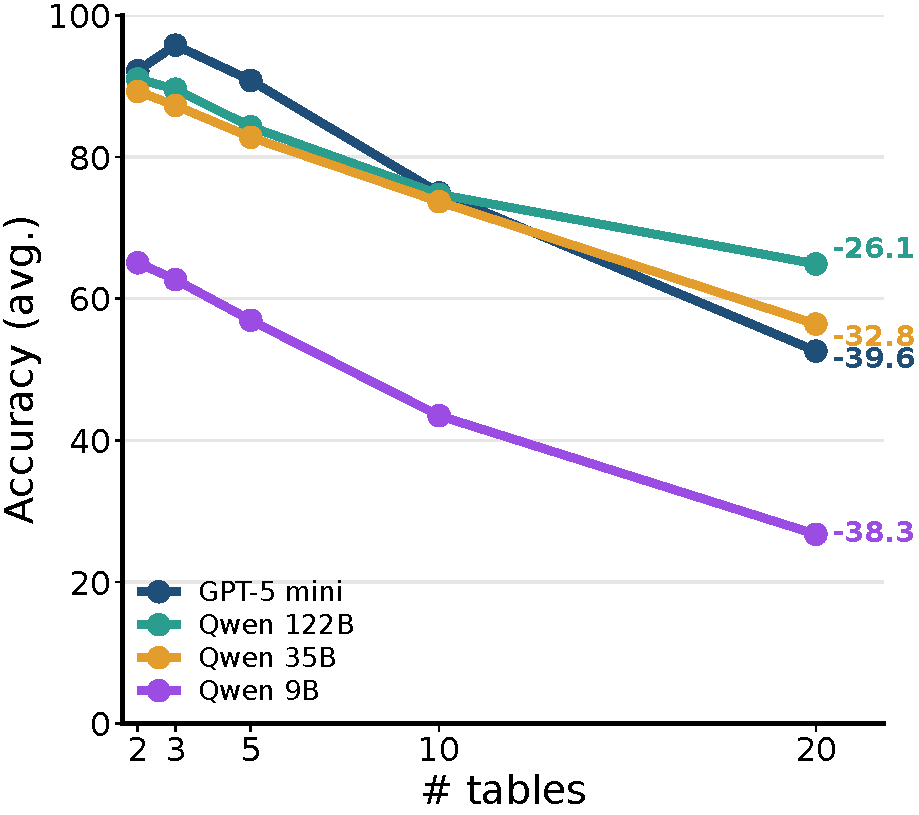
\includegraphics[width=\linewidth]{img/scaling_parallel.pdf}
        \caption{Parallel questions}
        \label{fig:parallel_scaling}
    \end{subfigure}
    \hfill
    \begin{subfigure}[t]{0.32\textwidth}
        \centering
        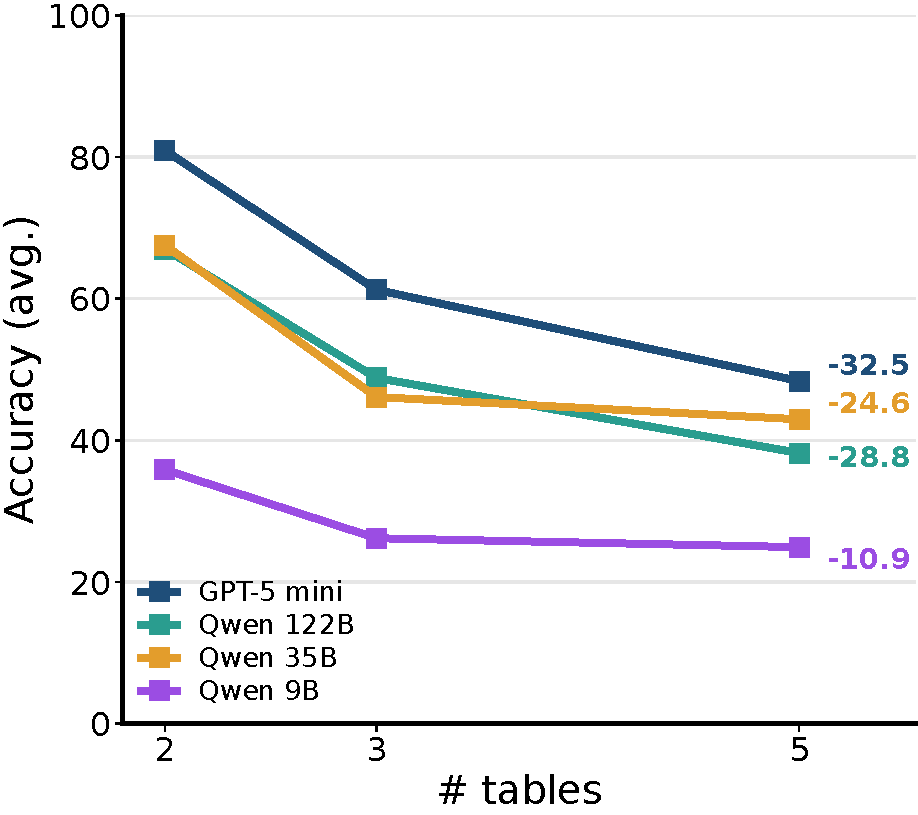
\includegraphics[width=\linewidth]{img/scaling_sequential.pdf}
        \caption{Sequential questions}
        \label{fig:sequential_scaling}
    \end{subfigure}
    \hfill
    \begin{subfigure}[t]{0.32\textwidth}
        \centering
        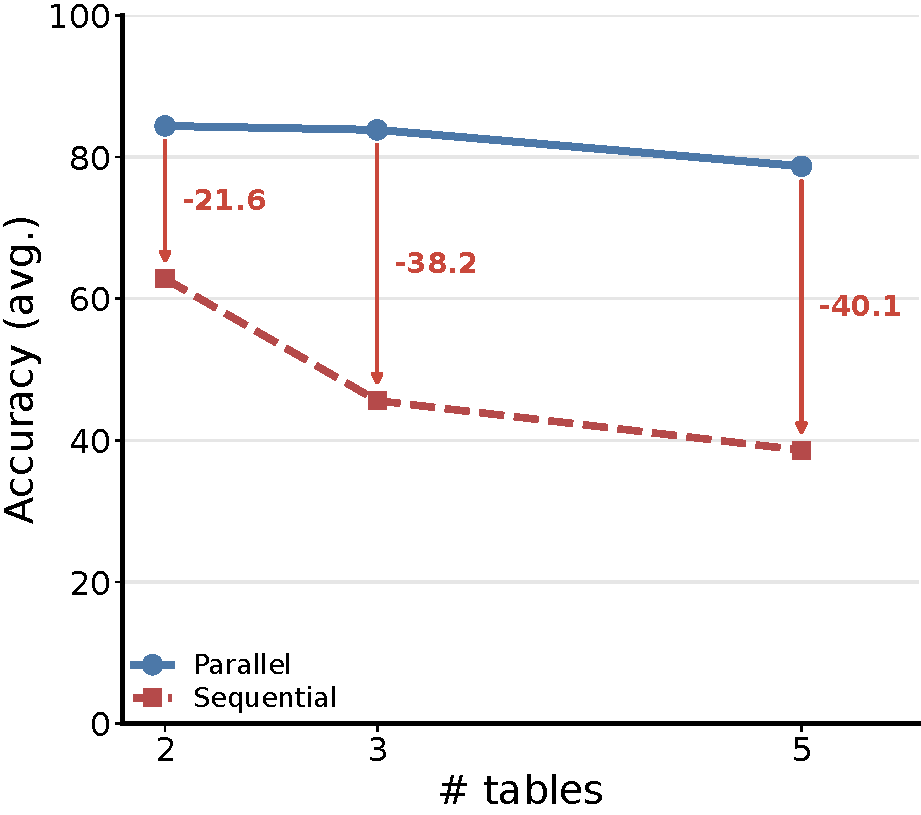
\includegraphics[width=\linewidth]{img/par_vs_seq.pdf}
        \caption{Parallel vs sequential}
        \label{fig:parallel_sequential_penalty}
    \end{subfigure}
    \caption{
    Scaling behavior as the number of tables increases.
    Labels at the end of curves in (a) and (b) report the accuracy drop from the smallest to largest table count.
    Panel (c) compares parallel and sequential questions at matched table counts, showing that sequential reasoning adds degradation beyond multi-table aggregation.
}
    \label{fig:scaling_parallel_sequential}
\end{figure*}

\subsection{Rendering Non-Relational Views}
\label{subsec:transformations}
Rendering is organized as an answer-preserving transformation sequence. Formally, rendering is a mapping
\begin{equation}
    \mathcal{R} : (S,\mathcal{P}) \mapsto \{V_1,\dots,V_k\},
\end{equation}
where each V_i is a non-relational view and \mathcal{P} is the provenance mask indicating cells required by the SQL program and cells safe to perturb.

\begin{definition}[Provenance mask]
A provenance mask \mathcal{P} is a Boolean annotation over cells of S such that \mathcal{P}(c)=\text{true} iff cell c is required to reconstruct the gold label under the given SQL supervision.
\end{definition}

\name first creates table-specific relational projections from the latent source and records a provenance mask marking cells required by the SQL program and cells safe to perturb. It then introduces null values, and applies column merging, unit rendering and conversion while the representation is still relational. Next, \name converts each projection into a non-relational view through a pivot-style transformation, organizing selected attributes as hierarchical row and column headers. The generator searches over candidate row/column partitions, prefers dense pivots, shrinks the layout, and retains all evidence required by the SQL program. Rendered views are capped at a user-specified size. After layout construction, \name inserts perturbations such as blank rows or columns, typographical noise, and contextual or footnote-like text.

\begin{proposition}[Answer preservation under rendering]
If \mathcal{R} is applied to (S,\mathcal{P}) and the provenance mask \mathcal{P} is honored (no required cell is deleted or irreversibly corrupted), then executing the original SQL supervision Q on S yields the same gold answer as computing the aggregation from the rendered views using the intended per-view extractive queries.
\end{proposition}

The same rendering machinery supports both multi-table regimes, with scenario-specific controls. In parallel generation, each view provides one independently retrievable scalar for the final aggregation, and unit conversion can force normalization across compatible quantities. In sequential generation, each view represents one step of a latent lookup chain. Intermediate views contain exactly one occurrence of the lookup key extracted from the previous view. This is an evaluation choice rather than a framework limitation: ambiguous or tree-shaped joins would add uncontrolled variation in join complexity and the number of values entering the final aggregation. Unique matches keep the reasoning depth comparable across instances while still requiring models to recover implicit cross-table links, since latent joins are not stated in the question. Finally, view order is randomized to prevent shortcutting. 
Overall, rendering hides clean schemas, explicit joins, and standardized numerical expressions while preserving verifiability through the latent relational source and SQL supervision.
\eat{
\fg{To construct the input given to the evaluated LLM, \name renders the latent relational source as non-relational views.} These transformations are answer-preserving: \name tracks the cells required by the SQL program and prevents perturbations from deleting or corrupting the evidence needed to recover the gold label.
We first apply schema-level changes, such as replacing synthetic attribute names with longer web-style headers and optionally merging columns. We then render measurement units either in headers or directly inside cells. Next, we convert flat tables into non-relational layouts through a pivot-style transformation that organizes selected attributes as hierarchical row and column headers. The generator searches over candidate row/column partitions, prefers dense pivots, and shrinks the resulting layout while ensuring that all evidence cells required by the latent SQL program are retained. \fg{In all experiments, rendered views are capped at $10 \times 10$ cells to keep inputs compact.} This is the main mechanism by which \name produces nested headers and non-trivial table layouts.
After layout construction, we apply cell- and structure-level perturbations, including blank rows and columns, null-like fillers in non-answer cells, typographical noise, and contextual or footnote-like text inserted into cells.  The same transformation machinery is used for both multi-table regimes, with additional scenario-specific controls.
For parallel generation, each non-relational view contains one independently retrievable scalar contribution to the final aggregation. Moreover, \name\ can optionally convert units inside each tabular view, forcing models to normalize compatible quantities across heterogeneous surface forms.
For sequential generation, each non-relational view contains one step of a latent lookup chain, so that solving the question requires propagating information across views before computing the final answer. Moreover, we constrain each intermediate view to contain exactly one occurrence of the lookup key extracted from the previous view.
This is an evaluation choice rather than a framework limitation: ambiguous or tree-shaped joins would introduce uncontrolled variation in both join complexity and the number of values entering the final aggregation.
By enforcing unique intermediate matches, we keep the reasoning depth comparable across instances while still requiring models to recover implicit cross-table links, since the latent joins are not stated in the question.
Finally, we randomize the order of sequential views to prevent models from using input order as a shortcut for the lookup chain.
Overall, this transformation stage yields benchmark instances that no longer expose a clean relational schema, explicit joins, or standardized numerical expressions, while still remaining fully verifiable. 
\mpaga{La parte precedente non può essere riscritta con il seguente ordine o è necessaria una precedenza tra le trasformazioni, adesso mi sembra un po' confusionaria? 1) Pivoting, 2) Trasformazioni allo schema (sinonimi e merging), 3) Trasformazioni sui valori: noise sui valori (null, typos, inline text) + conversione dei valori (w.r.t. meas. unit), 4) constraint enforcing (solo per sequential)} \mlc{non è reso esplicito, ma dal punto di vista implementativo applichiamo alcune trasformazioni sulla view relazionale per: proteggerci da eventuali perturbazioni lossy (e.g. l'introduzione dei nan richiede una mask sulla tabella relazionale che ci indichi quali celle possiamo rendere nan), impossibilità di perturbazioni post-pivot (column merging sarebbe difficile, in quanto non sapremmo bene come unire righe che possono variare su molteplici livelli di header di riga/colonna: è più semplice farlo su tab. relazionale. Stessa cosa per unità di misura, a cui inoltre inseriamo l'unità di misura in maniere diverse: nelle celle, nell'header di colonna, in una cella in alto a sinistra nella tabella). Altre perturbazioni più semplici e locali (e.g. typo) le facciamo post pivot.}}

\subsection{Question Verbalization and Verification}
\label{subsec:nl-generation}
In the final stage, \name\ prompts an LLM to generate a natural-language question. The prompt receives all 
non-relational views in HTML form, the SQL supervision, the aggregation description, and the gold answer. 

\begin{definition}[Verbalization function]
The verbalization function \mathcal{V} maps ( \{V_i\}, Q, y ) \mapsto q_\text{NL} where q_\text{NL} is a natural-language question whose intended interpretation corresponds to Q and y.
\end{definition}

The multi-table verbalization differs slightly across the two reasoning regimes. For parallel questions, the generator verbalizes the shared selection pattern together with the cross-table aggregation to be performed. For sequential questions, the generator verbalizes only the first and last steps of the chain and leaves intermediate dependencies implicit in the table contents. As a result, the final question does not expose the latent composition directly, but still requires the evaluated LLM to recover it from the views. To filter out noisy generations, we perform an LLM-based verification pass after question generation, repairing the NL question whenever the verbalization is inconsistent with the underlying supervision.

\begin{proposition}[Verification soundness]
If the LLM-based verifier accepts q_\text{NL} given (\{V_i\},Q,y), then q_\text{NL} is consistent with the SQL supervision Q and the gold answer y up to verifier accuracy.
\end{proposition}

\eat{In the final stage, \name\ prompts an LLM to generate a natural-language question. The prompt receives the 
non-relational views in HTML form, the SQL supervision, the aggregation description, and the gold answer. The wording is therefore conditioned on the exact evidence and operation required by the instance.
The multi-table verbalization differs slightly across the two reasoning regimes. For parallel questions, the generator verbalizes the shared selection pattern together with the cross-table aggregation to be performed. For sequential questions, the generator verbalizes only the first and last steps of the chain and leaves intermediate dependencies implicit in the table contents. As a result, the final question does not expose the latent composition directly, but still requires the model to recover it from the views. To filter out noisy generations, we perform an LLM-based verification pass after question generation. The verifier receives the generated question, the supporting views, the latent SQL program, and the gold answer, and updates the question whenever the verbalization is inconsistent with the underlying supervision. 
} 
